\documentclass{minmal}
\usepackage[utf8]{inputenc}
\usepackage{amsmath, amssymb}
\usepackage{graphicx}
\usepackage{geometry}
\geometry{margin=2.5cm}
\usepackage{hyperref}
\usepackage{caption}
\usepackage{float}
\usepackage{tikz, pgfplots}
\pgfplotsset{compat=1.18}
 
\title{Lambda-metoden ($\lambda$-tuning) for PI-regulatorer}

\date{\today}
\author{Svein-Tore Narvestad}
 
\begin{document}
\maketitle
\section{Introduksjon}
Når man arbeider med styressystemer i industrien så er det viktig at man har regulatorer med gode regulatorparametre ($K_p$,$T_i$ og $T_d$).  Har man gode parametre kan en regulering se slik ut:
\begin{figure}[H]
    \centering
    
\includegraphics[width=0.5\linewidth]{prosessfag/bilder/optimal_regualtor.png}
\end{figure}
\noindent Men om vi har feil parametre så kan det bli veldig feil.  her kan du se et eksempel på det:\nl
\begin{figure}[H]
    \centering
    
\includegraphics[width=0.5\linewidth]{prosessfag/bilder/regulator_kaos.png}
\end{figure}
\noindent Vi har tidligere sett på hvordan vi kan optimalisere en prosess med Ziegler-Nichols metode.  Denne gir gode resultater. Men det å øke $K_P$ verdien til man får stående svingninger er noe man sjeldent får til. I hvert fall i virkelige prosessanlegg, som vi skal jobbe med nå.  Et alternativ til denne er Lambda metoden. Lambda-metoden (også kjent som Skogestad-metoden) er en modellbasert metode for å stille inn PI- og PID-regulatorer. Metoden er spesielt nyttig for industrielle prosesser som kan beskrives som førsteordens systemer med tidsforsinkelse (FOPDT), for eksempel tankanlegg, temperatur- strømningsmengde- eller nivåprosesser.  Metoden går ut på at man setter regulatoren i manuell.  Så gjør man en endring (manuelt) i pådragsorganet (f.eks 10\%).  Om vi gjør det vil for den regulerte størrelse få en endring veldig likt kurven under:\nl
\begin{figure}[H]
\centering
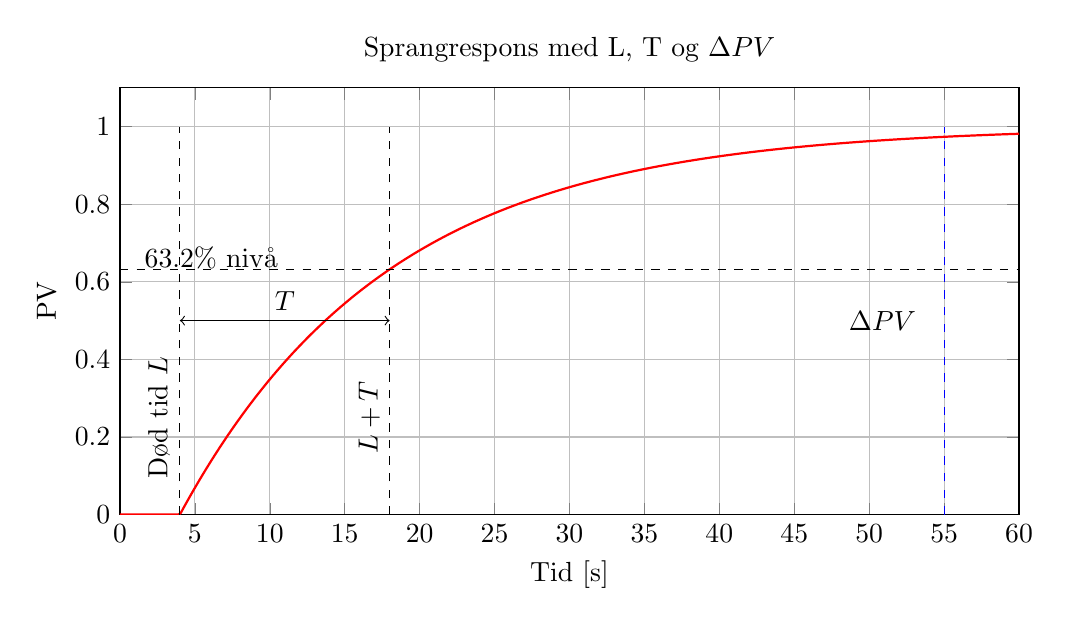
\begin{tikzpicture}
\begin{axis}[
    width=13cm,
    height=7cm,
    xlabel={Tid [s]},
    ylabel={PV},
    xmin=0, xmax=60,
    ymin=0, ymax=1.1,
    grid=both,
    title={Sprangrespons med L, T og $\Delta PV$},
]

% --- Parameters ---
\def\L{4}
\def\T{14}
\def\K{1}

% --- FOPDT response curve ---
\addplot[
    thick,
    red,
    domain=0:60,
    samples=400,
]
{ (x < \L) * 0 + (x >= \L) * (1 - exp(-(x-\L)/\T)) };

% --- Mark L ---
\addplot[dashed] coordinates {(\L,0) (\L,1)};
\node[rotate=90, anchor=south] at (axis cs:\L,0.25) {Død tid $L$};

% --- Mark L+T ---
\pgfmathsetmacro{\LT}{\L + \T}
\addplot[dashed] coordinates {(\LT,0) (\LT,1)};
\node[rotate=90, anchor=south] at (axis cs:\LT,0.25) {$L + T$};

% --- 63.2% line ---
\pgfmathsetmacro{\ytau}{0.632}
\addplot[dashed] coordinates {(0,\ytau) (60,\ytau)};
\node[anchor=west] at (axis cs:1,\ytau+0.03) {63.2\% nivå};

% --- ΔPV marking ---
\addplot[dashed, blue] coordinates {(55,0) (55,1)};
\node[anchor=west] at (axis cs:48,0.5) {$\Delta PV$};
\draw[<->]
    (axis cs:\L,0.5)
    --
    (axis cs:\LT,0.5)
    node[midway, above] {$T$};
\end{axis}

\end{tikzpicture}
\end{figure}
I denne grafen er det flere verdier som er viktige for å finne optimale PID parametre.  Og det er død tiden (L), tidskonstanen (T) og prosessforstrerkningen (K) 
\section{Fremgangsmåte for Lambda-tuning}
 
\subsection{Identifisering av prosessparametre}
Gjennomfør et sprangforsøk på prosessen:
 
\begin{enumerate}
    \item \textbf{Sprangendring:} Du gjør en manuell positiv endring i pådraget $\Delta u$ på 10\%.  Så noterer du hvordan prosessresponsen blir.  Du må altså skrive ned verdien for prosessvariabelen (PV) for hvert sekund til den igjen stabiliserer seg. Styreystemet har mulighet for det.  Så lager du en graf som vist over av verdiene.  Til slutt estimerer du $K$, $T$, og $L$.
\end{enumerate}
 
Fra responsen kan du lese av:
\begin{itemize}
    \item \textbf{Død tid (L):} tidspunktet der prosessverdien (PV) først begynner å endre seg etter pådraget.
    \item \textbf{Tidskonstant (T):} tiden det tar for PV å nå 63,2\% av endringen etter forsinkelsen.
    \item \textbf{Prosessforsterkning (K):} $\Delta PV / \Delta u$.
\end{itemize}
 
\subsection{2. Valg av lukket sløyfe-tidskonstant (\texorpdfstring{$\lambda$}{lambda})}
Velg $\lambda$ avhengig av ønsket robusthet og respons:
\[
\lambda = L \quad (\text{rask respons})
\]
\[
\lambda = 3 L \quad (\text{moderat, robust})
\]
\[
\lambda = 5 L \quad (\text{rolig, stabil})
\]
 
\subsection{3. Beregning av PI-parametre}
For en PI-regulator:
\begin{equation}
K_p = \frac{T}{K (\lambda + L)}
\end{equation}
\begin{equation}
T_i = T + L
\end{equation}
 
\section{Praktisk gjennomføring på tankanlegg}
\begin{enumerate}
    \item Sett regulator i manuell modus.
    \item Utfør først et lite sprang og noter responsen.
    \item Utfør deretter et større sprang, mål PV over tid.
    \item Estimer $L$, $T$ og $K$ fra dataene.
    \item Velg $\lambda$ basert på ønsket robusthet og responstid.
    \item Beregn $K_p$ og $T_i$.
    \item Sett regulator i automatikk og test med små settpunktsendringer.
    \item Juster $\lambda$ om nødvendig for å få ønsket dynamikk.
\end{enumerate}
 
\section{Hvorfor lite sprang først?}
\begin{itemize}
    \item Avdekker ikke-linearitet i ventiler eller målere.
    \item Avdekker dødsoner og ventilslep.
    \item Reduserer risikoen for å tunere regulatoren basert på feil modell.
\end{itemize}
 
\section{Eksempel}
Anta en prosess med:
\[
K = 1, \quad T = 14\,\text{s}, \quad L = 4\,\text{s}
\]
Velg $\lambda = 3L = 12\,\text{s}$.
 
Da blir PI-parametrene:
\[
K_p = \frac{14}{1 \cdot (12 + 4)} = 0.875
\]
\[
T_i = 14 + 4 = 18\,\text{s}
\]
 
Dette gir en stabil og rolig regulering, egnet for tankprosesser.
 
\section{Figur}
\begin{figure}[H]
    \centering
    \begin{figure}[H]
\centering
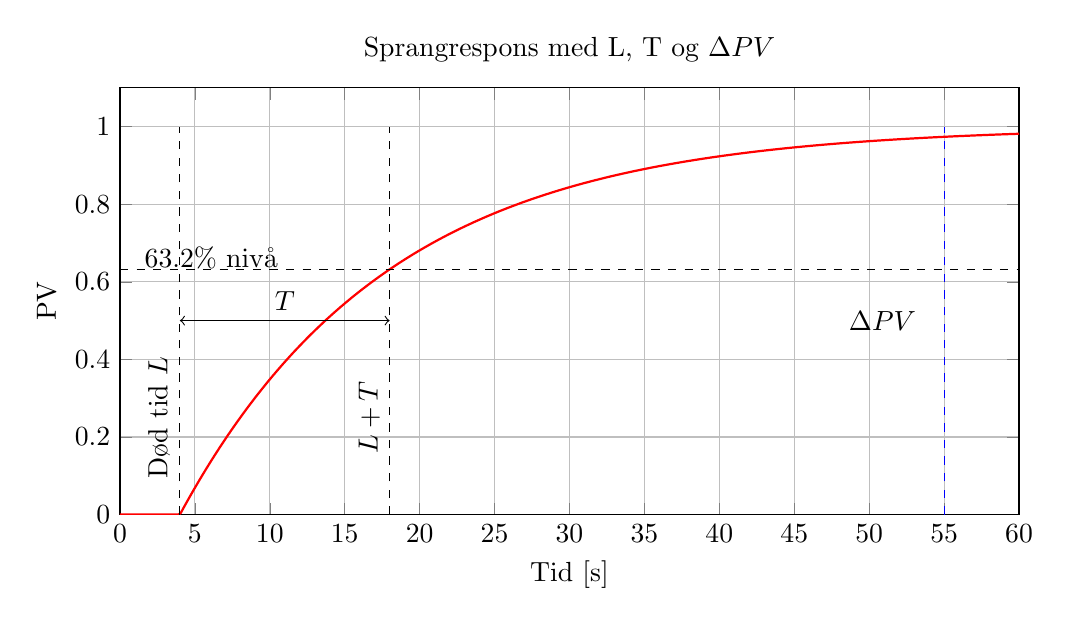
\begin{tikzpicture}
\begin{axis}[
    width=13cm,
    height=7cm,
    xlabel={Tid [s]},
    ylabel={PV},
    xmin=0, xmax=60,
    ymin=0, ymax=1.1,
    grid=both,
    title={Sprangrespons med L, T og $\Delta PV$},
]

% --- Parameters ---
\def\L{4}
\def\T{14}
\def\K{1}

% --- FOPDT response curve ---
\addplot[
    thick,
    red,
    domain=0:60,
    samples=400,
]
{ (x < \L) * 0 + (x >= \L) * (1 - exp(-(x-\L)/\T)) };

% --- Mark L ---
\addplot[dashed] coordinates {(\L,0) (\L,1)};
\node[rotate=90, anchor=south] at (axis cs:\L,0.25) {Død tid $L$};

% --- Mark L+T ---
\pgfmathsetmacro{\LT}{\L + \T}
\addplot[dashed] coordinates {(\LT,0) (\LT,1)};
\node[rotate=90, anchor=south] at (axis cs:\LT,0.25) {$L + T$};

% --- 63.2% line ---
\pgfmathsetmacro{\ytau}{0.632}
\addplot[dashed] coordinates {(0,\ytau) (60,\ytau)};
\node[anchor=west] at (axis cs:1,\ytau+0.03) {63.2\% nivå};

% --- ΔPV marking ---
\addplot[dashed, blue] coordinates {(55,0) (55,1)};
\node[anchor=west] at (axis cs:48,0.5) {$\Delta PV$};
\draw[<->]
    (axis cs:\L,0.5)
    --
    (axis cs:\LT,0.5)
    node[midway, above] {$T$};
\end{axis}

\end{tikzpicture}
\caption{TikZ-generert FOPDT-sprangrespons med markert $L$, $T$ og $\Delta PV$.}
\end{figure}
    \caption{Eksempel på sprangrespons i en tankprosess (ASCII eller simulert). Død tid $L$ og 63,2\% nivå brukes for å estimere $T$.}
\end{figure}
 
\section{Konklusjon}
Lambda-metoden gir en enkel og robust måte å stille inn PI-regulatorer på, spesielt for tregt dynamiske prosesser som tankanlegg. Den kombinerer modellbasert tuning med praktiske sprangforsøk for å identifisere prosessparametre. Ved å starte med et lite sprang først avdekkes ikke-linearitet, og et større sprang gir pålitelig identifikasjon av $K$, $T$ og $L$.
 \begin{figure}[ht]
\centering
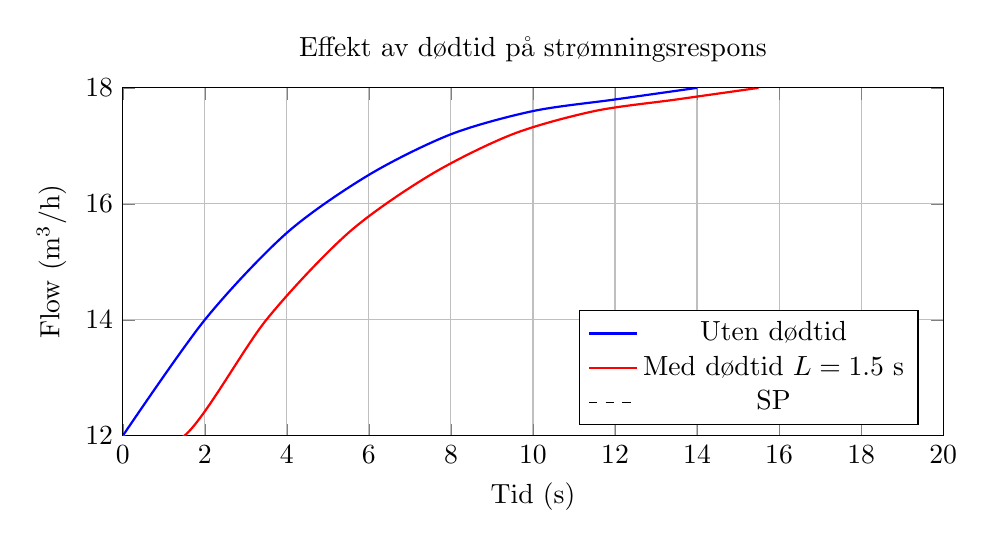
\begin{tikzpicture}
  \begin{axis}[
    width=12cm, height=6cm,
    xlabel=Tid (s),
    ylabel=Flow (m$^3$/h),
    xmin=0, xmax=20,
    ymin=12, ymax=18,
    grid=both,
    legend pos=south east,
    title={Effekt av dødtid på strømningsrespons}
  ]

  % Kurve uten dødtid
  \addplot[thick,blue,smooth] coordinates {
    (0,12.0)
    (2,14.0)
    (4,15.5)
    (6,16.5)
    (8,17.2)
    (10,17.6)
    (12,17.8)
    (14,18.0)
  };
  \addlegendentry{Uten dødtid}

  % Kurve med dødtid L=1.5 s
  \addplot[thick,red,smooth] coordinates {
    (0,12.0)
    (1.5,12.0)
    (3.5,14.0)
    (5.5,15.5)
    (7.5,16.5)
    (9.5,17.2)
    (11.5,17.6)
    (13.5,17.8)
    (15.5,18.0)
  };
  \addlegendentry{Med dødtid $L=1.5$ s}

  % Setpoint linje
  \addplot[dashed,black] coordinates {(0,18) (20,18)};
  \addlegendentry{SP}

  \end{axis}
\end{tikzpicture}
\caption{Strømningsprosessen med og uten dødtid. Dødtiden forsinker starten på responsen.}
\end{figure}

\begin{figure}[ht]
\centering
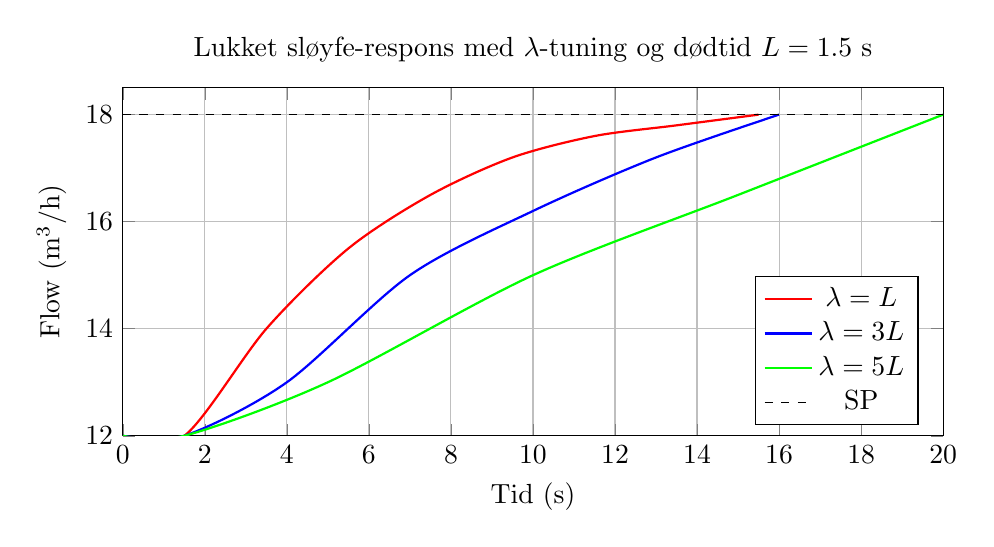
\begin{tikzpicture}
  \begin{axis}[
    width=12cm, height=6cm,
    xlabel=Tid (s),
    ylabel=Flow (m$^3$/h),
    xmin=0, xmax=20,
    ymin=12, ymax=18.5,
    grid=both,
    legend pos=south east,
    title={Lukket sløyfe-respons med \(\lambda\)-tuning og dødtid \(L=1.5\) s}
  ]

  % Rask lambda (λ=L)
  \addplot[thick,red,smooth] coordinates {
    (0,12.0) (1.5,12.0) (3.5,14.0) (5.5,15.5) (7.5,16.5) (9.5,17.2) (11.5,17.6) (13.5,17.8) (15.5,18.0)
  };
  \addlegendentry{$\lambda=L$}

  % Moderat lambda (λ=3L)
  \addplot[thick,blue,smooth] coordinates {
    (0,12.0) (1.5,12.0) (4.0,13.0) (7.0,15.0) (10.0,16.2) (13.0,17.2) (16.0,18.0)
  };
  \addlegendentry{$\lambda=3L$}

  % Rolig lambda (λ=5L)
  \addplot[thick,green,smooth] coordinates {
    (0,12.0) (1.5,12.0) (5.0,13.0) (10.0,15.0) (15.0,16.5) (20.0,18.0)
  };
  \addlegendentry{$\lambda=5L$}

  % Setpoint linje
  \addplot[dashed,black] coordinates {(0,18) (20,18)};
  \addlegendentry{SP}

  \end{axis}
\end{tikzpicture}
\caption{Sammenligning av aggressivitet ved ulike valg av \(\lambda\).}
\end{figure}
\end{document}